\section{Прикладная задача поиска оптимального управления}
\label{sec:optimal_cpntrol}
Задача глобальной оптимизации возникает при синтезе оптимальных с точки зрения некоторых
критериев управлений в линейных системах ОДУ. Если управление является линейной обратной
связью по состоянию, то система с управлением имеет вид:
\begin{equation}
  \label{eq:control_system}
    \dot x = (A+B_u\Theta)x + B_v v, x(0)=0,
\end{equation}
где  \(v(t)\in L_2\) --- некоторое возмущение.
Выходы системы описываются формулами \(z_k=(C_k+B_u\Theta),k=\overline{1,N}\).
Вляиние возмущения на \(k\)-й выход системы описывается критерием
\begin{displaymath}
  J_k(\Theta)=\sup_{v\in L_2} \frac{\max_{1\le i \le n_k} \sup_{t\ge 0}|z_k^{(i)}(\Theta,t)|}{||v||_2}.
\end{displaymath}

Нужно найти компоненты вектора \(\Theta\), минимизирующие один из критериев при
заданных ограничениях на другие:
\begin{displaymath}
   J_1(\Theta^*)=\min\{J_1(\Theta):J_k(\Theta)\leqslant S_k,k=\overline{2,N}\}.
\end{displaymath}

В \cite{optControl} указан способ вычисления критериев, состоящий в следующем:
\begin{itemize}
\item найти матрицу \(Y\) из уравнения:
\begin{displaymath}
  (A+B_u\Theta)Y+Y(A+B_u\Theta)^\mathsf{T}+B_v B_v^\mathsf{T} = 0
\end{displaymath}
\item если \(Y\) положительно определена, то используя её, вычислить функционалы \(J_k(\Theta)\):
\begin{displaymath}
  J_k(\Theta)=\sqrt{\max_{1\leqslant i\leqslant n_k}\{(C_k^{(i)}+D_k^{(i)}\Theta)Y(C_k^{(i)}+D_k^{(i)}\Theta)^\mathsf{T}\}},k=\overline{1,N},
\end{displaymath}
где \(C_k^{(i)},D_k^{(i)}\) --- \(i\)-е строки матриц \(C_k\) и \(D_k\) соответственно.
\end{itemize}

Для предотвращения случаев, когда \(Y\) незнакоопределена, в качестве дополнительного ограничения
использовался критеий устойчивости линейной системы ОДУ: все действительные части
собственных чисел матрицы \(A+B_u\Theta\) должны быть отрицательны:
\begin{displaymath}
  g_0(\Theta)=\min_{j}\re(\lambda_j(\Theta)) < 0
\end{displaymath}

На текущий момент с целью проверки корректности реализации вычисления критериев задачи
индексным алгоритмом глобального поиска были решены две задачи рассматриваемого типа
(их решение также приведено и в \cite{optControl}).
Описание индексной схемы учёта ограничений для метода из раздела (\ref{sec:method}) можно
найти в \cite{strongSerg}.

В задаче виброзащиты параметры системы (\ref{eq:control_system}) определются следующим
образом:
$$
A=\begin{bmatrix}
    0       & 1 \\
    0       & 0 \\
\end{bmatrix},
B_v=B_u=\begin{bmatrix}
  0       \\
  1       \\
\end{bmatrix},
C_1=\begin{bmatrix}
  0     & 1
\end{bmatrix},D_1=0,
C_2=\begin{bmatrix}
  0     & 1
\end{bmatrix},D_2=1.
$$

Управление имеет вид \(u=[\theta_1,\theta_2]x\), где \(\theta_1 \leqslant 0,\theta_2\leqslant 0\) ---
оптимизируемые параметры. Сама задача ставится следующим образом:
\begin{displaymath}
   J_2(\Theta^*)=\min\{J_2(\Theta):J_1(\Theta)\leqslant 1, g_0(\Theta)\leqslant -0.02\}.
\end{displaymath}

\begin{figure}[ht]
  \center
  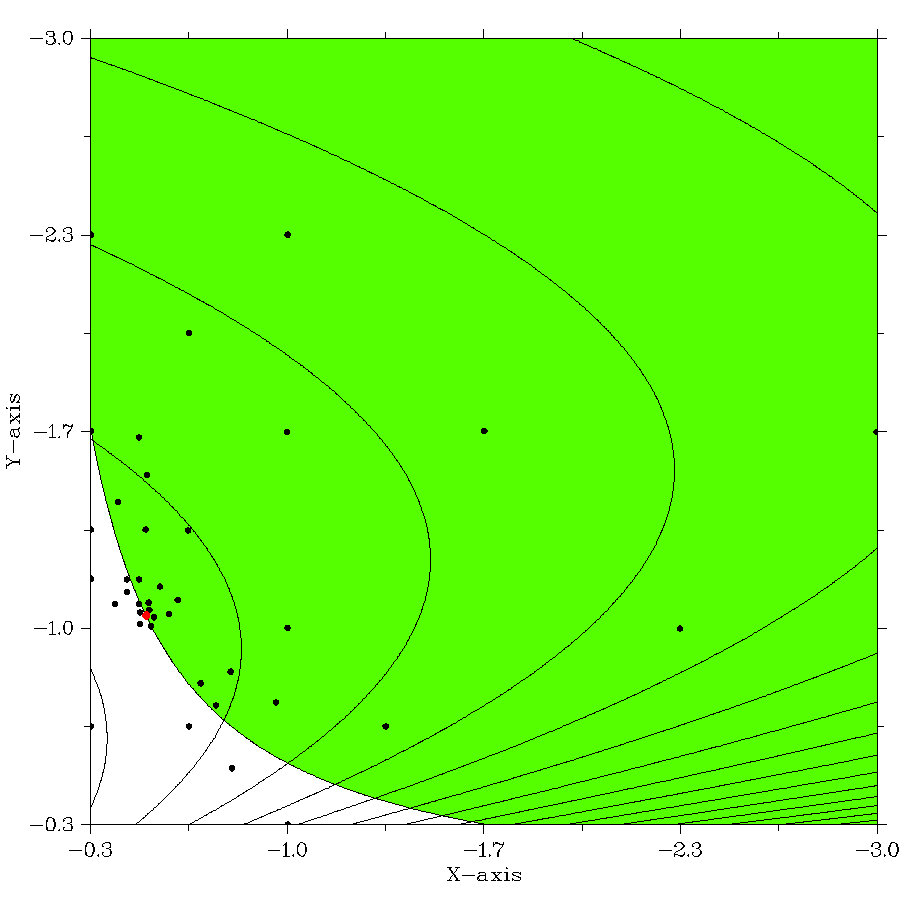
\includegraphics[width=0.55\textwidth]{images/controlProblem.png}
  \caption{Линии уровня для задачи виброзащиты с отмеченными точками испытаний АГП}
  \label{fig:controlProblem}
\end{figure}
При решении этой задачи АГП с параметрами \(r=2.3\), \(\varepsilon=10^{-2}\) произвёл
65 испытаний, причём целевая функция была вычислена 27 раз. Найдена оптимальная точка с координатами
\(\widetilde\theta_1 =-0.503223,\widetilde\theta_2=-0.997168\), а \(J_2(\widetilde\Theta)=0.866551\).
На рис. \ref{fig:controlProblem}
представлены линии уровня целевой функции задачи виброзащиты. В данном случае допустимая область (закрашена на рисунке)
имеет довольно простую границу, а целевая функция унимодальна.

В задаче гашения колебаний параметры системы (\ref{eq:control_system}) определются следующим
образом:
$$
A=\begin{bmatrix}
  0  & 0 & 1 & 0 \\
  0  & 0 & 0 & 1 \\
  -2  & 1 & -2\beta & \beta \\
  1  & -1 & \beta & -\beta \\
\end{bmatrix}, \beta = 0.1,
B_v=\begin{bmatrix}
0       \\
0       \\
1       \\
1       \\
\end{bmatrix},
B_u=\begin{bmatrix}
0       \\
0       \\
0       \\
1       \\
\end{bmatrix},
$$
$$
C_1=\begin{bmatrix}
1 & 0 & 0 & 0 \\
-1 & 1 & 0 & 0
\end{bmatrix},
D_1=\begin{bmatrix}
0 \\
0
\end{bmatrix},
C_2=\begin{bmatrix}
0 & 0 & 0  & 1
\end{bmatrix},D_2=1.
$$

Управление имеет вид \(u=[\theta_1,\theta_2, \theta_3,\theta_4]x\), где \(\theta_1,\theta_2, \theta_3,\theta_4\) ---
оптимизируемые параметры. Сама задача ставится так же, как и предыдущая:
\begin{displaymath}
   J_2(\Theta^*)=\min\{J_2(\Theta):J_1(\Theta)\leqslant 1, g_0(\Theta)\leqslant -0.02\}.
\end{displaymath}

В процессе решения этой задачи АГП c указанными ранее параметрами сделал 336575 испытания, причём целевая функция
была вычислена 5173 раза. Найдена оптимальная точка с координатами
\(\widetilde\theta_1 =0.322954,\widetilde\theta_2=-0.583130, \widetilde\theta_3=-0.453491, \widetilde\theta_4=-0.970581\),
а \(J_2(\widetilde\Theta)=1.056579\).
